%% lfsr.tex
%% 2012/07/24
%% by Max Lv

\documentclass[10pt,twocolumn,letterpaper]{article}

%% CVPR
\usepackage{cvpr}
\usepackage{times}
\usepackage{epsfig}
\usepackage{amsmath}
\usepackage{amssymb}

% Custom packages
\usepackage{multirow}
\usepackage{paralist}

% \cvprfinalcopy % *** Uncomment this line for the final submission

\def\cvprPaperID{****} % *** Enter the CVPR Paper ID here
\def\httilde{\mbox{\tt\raisebox{-.5ex}{\symbol{126}}}}

% Pages are numbered in submission mode, and unnumbered in camera-ready
\ifcvprfinal\pagestyle{empty}\fi

%% CITATION PACKAGES
\usepackage{cite}
\usepackage[pagebackref=true,colorlinks,bookmarks=false]{hyperref}

%% GRAPHICS RELATED PACKAGES
\usepackage{graphicx}

%% ALIGNMENT PACKAGES
\usepackage{array}

%% SUBFIGURE PACKAGES
\usepackage[tight,footnotesize]{subfigure}

% PDF, URL AND HYPERLINK PACKAGES
\usepackage{url}

% FIX FOR SPANNING
\usepackage{stfloats}

% description list
\newcounter{desccount}
\newcommand{\desclabel}[1]{%
  \refstepcounter{desccount}\label{#1}
}

% correct bad hyphenation here
\hyphenation{op-tical net-works semi-conduc-tor}

\makeatletter
\newcommand*{\rom}[1]{\expandafter\@slowromancap\romannumeral #1@}
\makeatother

%% DOCUMENT
\begin{document}

%% TITLE
\title{Local Feature Based Salient Region Detection}

%% AUTHOR
\author{
	\alignauthor
	Chao Lv\\
    Parallel Processing Institute\\
    Fudan University\\
    {\tt\small lch@fudan.edu.cn}
}

\maketitle

%% DOCUMENT BODY

\begin{figure*}[!t]
	\centering
	\subfigure[Salient region has the densest local features.]{
		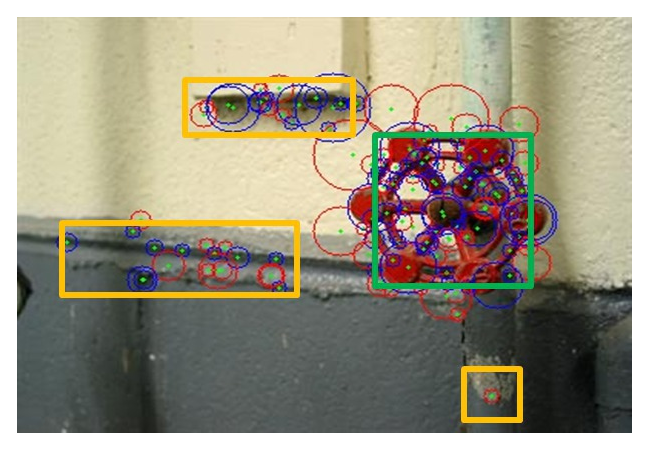
\includegraphics[width=2.5in]{images/fig-observation1.eps}
		\label{fig:observation_1}
	}
	\hfil
	\subfigure[Several salient regions in one image.]{
		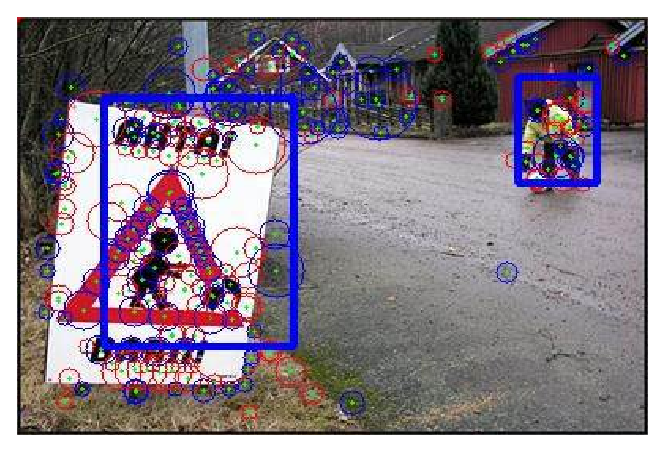
\includegraphics[width=2.5in]{images/fig-observation2.eps}
		\label{fig:observation_2}
	}
	\caption{Example images with local feature based salient regions}
	\label{fig:observations}
\end{figure*}

\begin{abstract}

Local feature descriptors have become the most important part in image / video retrieval systems. But considering the great amount of local features, thousands of local features in one HD photo, it's hard to compute them efficiently in a realistic system. 

To overcome this obstacle, we purpose a straightforward local feature reduction by using a algorithm named LFSR (Local Feature based Salient Region). With no additional computation for salient regions, this algorithm help to improve both the performance and accuracy of local feature descriptors. In our evaluation, we also compare LFSR algorithm with a state-of-the-art salient region algorithm~\cite{achanta2009frequency}. And the results shows that LFSR provides a thousands of times computation speedup, with an acceptable precision loss. Furthermore, when integrated with the SURF algorithm, LFSR can provide a overall 1.6X speedup.

\end{abstract}


\section{Introduction}

Our society has entered a data-centric era and a huge amount of data are transferred and processed on the Internet. Among them, multimedia data, such as image and video, has become one of the major data types being processed. As analyzed by CISCO Inc., video data occupies 50\% of network traffic in 2011 and will increase to 90\% in 2013~\cite{CISCO2011}.  According to a report~\cite{youtube2009}, as one of the most popular video sharing sites, more than 20-hour new videos are uploaded to \emph{YouTube} every minute. Moreover, as two most popular photo sharing sites, \emph{Facebook} and \emph{Flickr} host billions of user-uploaded images respectively.

With the rapid increase of multimedia data, one of the most significant challenges is to understand and interpret such a huge amount of multimedia data. Currently, more and more retrieval applications are emerging to process these multimedia data, such as video recommendation~\cite{videorecommendation2007}, travel guidance systems~\cite{travelguidance2010} and content-based TV copy identification~\cite{tvidentify2003}. In these systems, a fundamental step is to extract feature information from images. 

Image features can be divided into two domains -- local features and global features. Global image features tend to describe the image as a whole, such as contour representations, shape descriptors and texture features. On the other hand, local image features represent image patches, computed at multiple points in the image. For example, SIFT~\cite{Lowe2004SIFT} and SURF~\cite{Bay2006SURF} are two most widely-used local image feature descriptors~\cite{Mikolajczyk2005Evaluation}\cite{Bauer2007Evaluation}. They use histograms of gradient orientations to extract feature points and describe them using high-dimension feature vectors.

Compared to the global features, local feature descriptors are more robust, both scale-invariant and rotation-invariant. But even the SURF descriptor, which is an optimized algorithm for SIFT, is still very slow in a practical usage -- the processing speed of SURF is about 2.6 frame per second on a 3.3GHz Core i7 CPU~\cite{Fang2011ispass}, far from the requirement of real time. Actually local feature descriptor should extract enough feature points from one image, and these features can be more than thousands in a standard VGA ($640\times480$) image. Considering the computation for describing each local feature, the great amount of local features means a relatively high overhead.

In general, there exist three major computation phases when processing local image features in a typical image retrieval system. First, the system detect all feature points from images. Then, with some specific formats and algorithms, each feature point is described as a high dimension vector. At last, all extracted feature are compared to each other according to the distance of their vectors.

According to a previous research~\cite{Fang2011ispass}, the computation of feature describing are obviously greater than the feature detecting in the SURF algorithm, which is caused by the great amount of local features to be described in one image. Furthermore, in a realistic image retrieval system, the performance is dominated by the number of features in the database.

So, it's possible and necessary to improve the performance of the whole system by the reduction of local features extracted from each image. In this paper, we present a algorithm named LFSR (Local Feature based Salient Region) to eliminate unimportant local features efficiently with no obvious precision loss for a image retrieval system.

The main idea of LFSR algorithm is extracting salient regions of images and only describing the local features in those regions. Without involving any other salient region algorithm, it is only based on the feature points extracted from the first phase of a typical local feature algorithm. This approach has two remarkable advantages: no additional computation for salient region detection; totally integrated with local feature algorithm to compute the salient region efficiently. The details of LFSR can be found in Section 2. 

We have evaluated LFSR against a stat-of-the-art salient region algorithm. The evaluation results show that our approach has a much better performance with compatible precision and recall. Furthermore, withing a realistic image retrieval system, our evaluation shows that LFSR can help to improve both performance and accuracy.

\section{Observations}

We propose LFSR algorithm based on three observations:

\begin{itemize}
	
	\item {\bf Observation 1:} Local feature in the salient region are close to each other, while noisy or unimportant features are far away from them. As shown in Figure \ref{fig:observation_1}, local features in the salient region (green box) gather together and many obvious unimportant local features locate far from that box.

	\item {\bf Observation 2:} The region with most local features is the preferred salient region. Also from Figure \ref{fig:observation_1}, the preferred green box has much more local features than in other two yellow boxes.

	\item {\bf Observation 3:} There may exist several salient regions in one image. For example, the photo in Figure \ref{fig:observation_2} contains two objects, a person and a stop sign, which shape two salient region following the distribution of local features on them.

\end{itemize}

Observation 1 indicates a method to rewrite our a

\section{{\sys} Algorithm}
\label{sec:algorithm}

\subsection{Overview}
\label{sec:algorithm_overview}

\begin{figure*}[!ht]
\centering
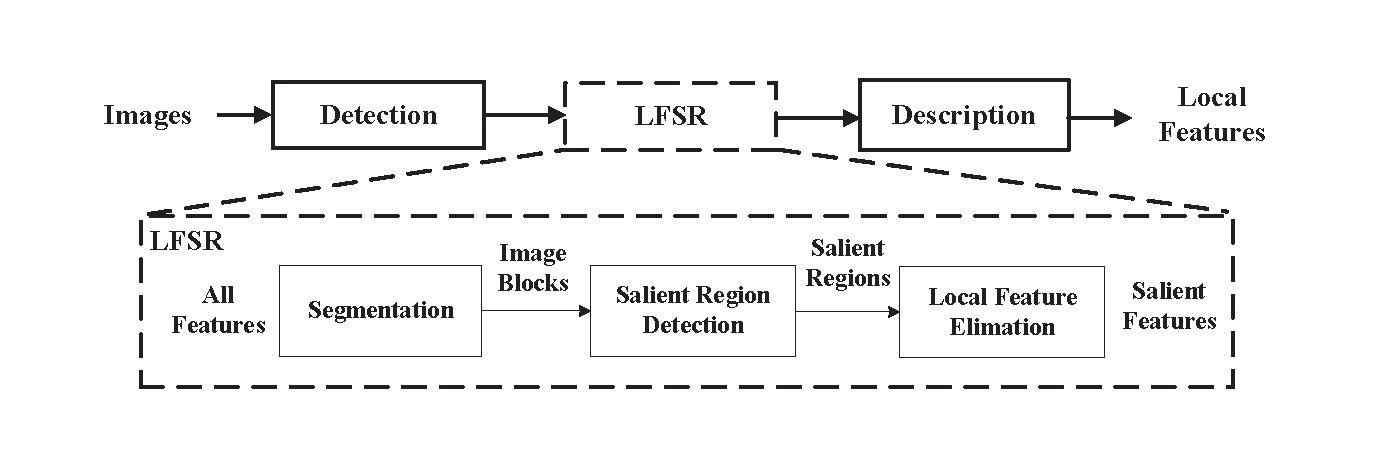
\includegraphics[width=4.5in]{images/fig-overview.eps}
\caption{An overview of {\sys}}
\label{fig:overview}
\end{figure*}

The basic motivation of {\sys} is to design a salient region detection algorithm, which can be used to optimize the obstacles of {\lfea}s and is easy to combined with them. Based on the observations in Section~\ref{subsec:observation}, we design and implement a local feature based salient region algorithm~({\sys}), which is efficient and easy to be combined with {\lfea}s.    

As shown in Figure \ref{fig:overview}, {\sys} works as a filter just between detection stage and description stage of a typical {\lfea}, where the input of {\sys} is detected feature points and its output is the sets of concerned feature points for computing feature vectors. There exist two major stages in our algorithm.
\begin{inparaenum}[\itshape a\upshape)]
\item First, a segmentation step is performed on all local features to identify and partition multiple salient region in an image. 
\item Second, for each image segmentation, {\sys} computes that segmentation's salient region individually based on the distribution information of the local feature points in it.
\end{inparaenum}


\subsection{Local Feature Based Segmentation}
\label{sec:algorithm_segmentation}

According to Observation~\ref{itm:observation_2}, an image may include several salient regions, which form multiple clusters of local features. We solve this problem by using a simple segmentation algorithm to divide the image into several blocks based on the distribution of local features. It scans along both the x axis and the y axis. In each scan, a cut-point may be found under the following two constraints:

\squishlist
\item \textit{No local feature could be divided into multiple parts.} In {\lfea}s, scale information is computed to guaranteed scale invariant. Therefore, a local feature point is used to represent a region with a radius that equals its scale as shown in Figure~\ref{fig:segmentation}. When the image is partitioned, no segmentation should across the region that a feature point representing.

\item \textit{The cut point should not locate far away form the center.} Each scan is performed from the region center. When the scan goes far, for example 1/4 of the region width, the scan stops and declares that there is no valid cut in that scan. This constraint attends to keep segmentation balanced and avoid too large or too small regions.
\squishend

A typical segmentation is shown in Figure~\ref{fig:segmentation}. The segmentation is started from the center of each axis, e.g. the dot lines in the figure. When a cut-point satisfying the above two constraints is found, The algorithm stops scanning and takes that cut-point as a valid image segmentation, e.g. the solid lines in the figure. After scanning on both the x axis and the y axis, at most four image regions are found in one segmentation.

\begin{figure}[!ht]
\centering
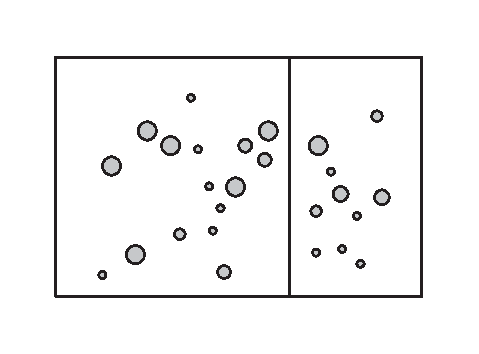
\includegraphics[width=2.1in]{images/fig-segmentation.eps}
\caption{Segmentation by scanning along both the x-axis and y-axis and starting from the dot lines and stops on the solid lines.}
\label{fig:segmentation}
\end{figure}

Then this kind of segmentation will be performed recursively on each image regions. And a recursive segmentation should stop when the following situations are satisfied:

\squishlist
\item \textit{No valid cuts are found.} When no valid cuts following the above two constraints are found, for example a scan exceeds its distance limit, on both x-axis and y-axis of a region, we should regard this region as a whole object and stop performing segmentation on it.

\item \textit{Too few features exist in a region.} Some found regions may have no local feature or just a few features, such as one or two local features, like gray regions in Figure~\ref{fig:segmentation-2}. These regions will be marked as invalid, because they cannot hold one whole object, and no further computation will be performed on them.

\item \textit{The number of segmentations exceeds the limitation.} It's possible that the recursive segmentation becomes too deep if there exist many dispersive points in that region. And actually it makes no sense to perform segmentation on these points, since they cannot be regarded as valid objects individually.

\squishend

\begin{figure}[!ht]
\centering
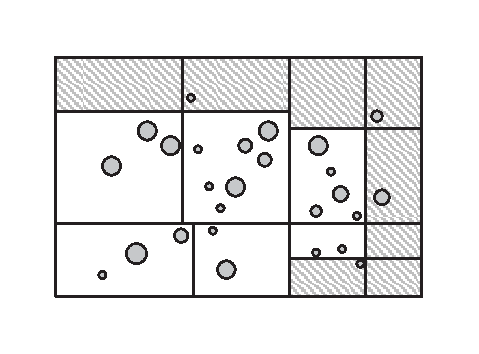
\includegraphics[width=2.1in]{images/fig-segmentation-2.eps}
\caption{Valid and invalid regions after two runs of segmentations. White regions are valid and gray regions are invalid.}
\label{fig:segmentation-2}
\end{figure}


According to our evaluation, in most cases two runs of segmentation are just enough, since almost no image has more than sixteen major objects. Thus, it's possible to simplify this processing by performing segmentation only twice in realistic scenarios.

\subsection{Salient Regaion Detection}
\label{sec:algorithm_detection}

As discussed in Section~\ref{sec:algorithm_overview}, a precise salient region detection is not suitable for local feature reduction in terms of processing speed and accuracy. Thus, {\sys} employs geometric meaning of local features to compute approximate salient regions.

According to Observation~\ref{itm:observation_1}, the local features in one salient region locate near to each other while noise or unimportant feature points locate far away from them. To simplify this problem, we regard the geometric center of feature points as the center of a salient region. Thus, the region center can be calculated based on the following equation:

{\begin{equation} \label{eq:center}
\left({x}_{c},{y}_{c} \right) = \frac{\sum_{i}^{N}\left({x}_{i},{y}_{i} \right)}{N}
\end{equation}}

Where $\left({x}_{c},{y}_{c} \right)$ means the geometric center of each local feature $\left({x}_{i},{y}_{i} \right)$ in that image segmentation.

After locating the center, we build the final salient regions by expanding the region as a rectangle with a particular width-length ratio. This ratio should be consistent with the distribution of local features, since local features always locate following the shape of target objects. Approximately, this ratio can be considered to equal to the ratio of the dispersion degree on x-axis and y-axis. For example, the bigger dispersion degree of local features on x-axis is, the bigger width-length ratio we will get. To compute the ratio of feature dispersions, we can divide the standard deviation of local feature position on x-axis by on y-axis:

{\begin{equation} \label{eq:ratio}
ratio = \sqrt{\frac{\sum_{i}^{N}\left ( x_{i}-x_{c} \right )^{2}}{\sum_{i}^{N}\left ( y_{i}-y_{c} \right )^{2}}}
\end{equation}}

Where $x_{i}$ and $y_{i}$ is a feature's position, while $x_{c}$ and $y_{c}$ is the center position computed by Equation~\ref{eq:center}. To get the final salient region, {\sys} grows the region size until the amount of local feature in it exceeds a desirable number, for example 50 percent of the original local features. As discussed in Observation \ref{itm:observation_3}, this threshold is important for providing a large enough salient region to avoid filtering local features on objects' edges and corners. In our evaluation, we find a ratio about 40\% is proper for most cases.

Combined with segmentation discussed in Section~\ref{sec:algorithm_segmentation}, the processing results will provide several candidate regions. According to Observation \ref{itm:observation_2}, we pick up the candidate regions that have at least 2 local features inside and regard them as the final salient regions.

\subsection{Local Feature Elimination}
\label{sec:algorithm_elimation}

With the knowledge of salient regions in an image, all features locate inside salient regions are kept for further computation, and all other features outside are just dropped. As a result, we get much fewer salient features in the local feature description stage, which can help to improve the whole algorithm's efficiency obviously.



\section{Related Work}

There exist many kinds of {\lfea}. SIFT~\cite{lowe1999object}\cite{lowe2004distinctive} is the most publicly accepted and robust {\lfea}. For different conditions or purposes, some variants of SIFT are also widely used, such as RIFT~\cite{lazebnik2005sparse}, GLOH~\cite{mikolajczyk2005performance}, and PCA-SIFT~\cite{ke2004pca}. To deal with the performance issue of SIFT, SURF~\cite{bay2006surf} is proposed in 2006 as an optimized local feature descriptor based on SIFT. With acceptable precision loss, SURF tends to be an efficient alternative of SIFT. Most of these algorithms are insensitive to various transformations, such as scaling, rotation and illumination.

Local feature descriptors are used widely because of their robustness. Some common applications include automatic image mosaic technique~\cite{yang2008image,salgian2007using}, panorama stitching~\cite{brown2003recognising,tang2008modified}, robot localization~\cite{se2001vision} and object recognition~\cite{heo2008illumination}. And most of them are sensitive to the computation time, or even require real time processing.

Most salient region researches focus on generating precise salient map. Some of them~\cite{cheng2011global,achanta2009frequency} have already achieved impressive precision and recall. Since salient region is really helpful to local feature descriptors, researchers have also tried to combine them together. Huang et al.~\cite{huang2009image} involves a salient region detection algorithm by Itti et al.~\cite{itti1998model} to eliminate nosies for SURF descriptor. Liang et al.~\cite{liang2010salient} uses similar salient map method to perform noise reduction for SIFT descriptor. But none of them try to reuse local features for salient region detection or consider improve the computation performance of local feature descriptors.

\section{Evaluation}
\label{sec:evaluation}

In this section, we first give out some comparisons on accuracy. Then, to show the performance improvement of local feature descriptor by using {\sys}, an evaluation is also performed on {\sys} combined with SIFT and SURF, two most widely used {\lfea}s.

These two evaluations are performed in two different environments. For salient region comparison, we run algorithms on a PC with one Intel Quad Core 2.4Ghz CPU. For image retrieval system integration, the {\sys} is integrated to an exist image retrieval system on a server with Intel Octa-Core i7 3.4Ghz CPU. We also employ two benchmarks for our evaluation. The first one is a dataset of 1000 $640\times480$images with labeling salient regions by Achanta et at.~\cite{achanta2009frequency}, which is used to evaluate the salient region accuracy. The second one is a much larger image database provided by Nist~\cite{nister-stewenius-cvpr-2006}, which consists of 10200 $640\times480$ images for benchmarking image retrieval system.

\subsection{Experimental Comparison}
\label{sec:evaluation_comparison}

The major motivation of this paper is to design an algorithm for local feature reduction using salient region. To achieve this goal, an approximate salient region detection algorithm is designed. Although our approach cannot detect precise salient region, we are still interested in evaluating its precision against general purpose ones. Here we compare {\sys} with GBSR (Global Contrast based Salient Region)~\cite{cheng2011global}. GBSR is a state-of-the-art salient region detection algorithm, which can achieve the best precision and recall rate compared with the other salient region algorithms. Moreover, it is written in C++, which makes us easy to compare the computation efficiency with ours. The processing time of GBSR includes two parts: the saliency map detection and its segmentation.

Since we only focus on local features, our precision and recall evaluation differs from regular salient region researches. As input, we first generate both SURF and SIFT local features for the whole dataset. Then we collect the feature points in the salient regions calculated by the ground truth (labeling regions also by Achanta et al.), GBSR and {\sys}. At last, the GBSR's and {\sys}'s precision and recall are calculated based on their results compared with that of the ground truth. In other words, only the local features computed by the ground truth are considered as the truly salient features and the others are false features. Thus, the precision and recall equations are defined as follows.

{\begin{equation} \label{eq:precision}
Precision = \frac{{N}_{correct}}{{n}_{detected}}
\end{equation}}

{\begin{equation} \label{eq:recall}
Recall = \frac{{N}_{correct}}{{N}_{true}}
\end{equation}}

Where ${N}_{correct}$ refers to the number of local features located in both the ground truth and GBSR or {\sys}. ${N}_{detected}$ in equation~\ref{eq:precision} refers to the total number of local features detected by GBSR or {\sys}, while ${N}_{true}$ in equation~\ref{eq:recall} is the number of truly salient features in the ground truth.

\begin{table}[!ht]
\begin{center}
\begin{tabular}{|l|c|c|c|c|c|}
\hline
 & P & R & RE & SM(ms) & SG(ms) \\
\hline
GBSR   & 0.81 & 0.86 & 39\% &180 & 2080 \\
{\sys} & 0.52 & 0.59  & 42\% & N/A & 3 \\
\hline
\end{tabular}
\end{center}
\caption{Comparison between GBSR and {\sys} in precision (P), recall (R), reduction efficiency, saliency map (SM) and segmentation (SG) processing time in milliseconds.}
\label{tab:comparison}
\end{table}

The comparison result is presented in Table~\ref{tab:comparison}. As shown in the column 2, 3 and 4, {\sys} gets lower precision rate and lower recall rate compared to GBSR. The major reason is that our algorithm is an approximate design, which focuses on fast processing speed and accurate retrieval instead of precise boundaries of salient regions. The reduction efficiency in the column 5 refers to the proportion of the left local features after a reduction. The results shows that both of them can help to eliminate more than half of the original features. GBSR achieves a higher reduction rate due to its precise boundary detection.

The result in the column 6 of Table~\ref{tab:comparison} presents the efficiency comparison, It shows that the well optimized GBSR costs average 2086 milliseconds to get the final salient region for an image, while {\sys} only costs 3.2 milliseconds. Even only counting the time for saliency map detection, GBSR still needs average 178 milliseconds. The performance result of {\sys} is very impressive but not surprising, because the computation of {\sys} is really simple and straightforward.

\subsection{Combination into Retrieval Systems}
\label{sec:evaluation_integration}

\begin{table}[!ht]
\begin{center}
\begin{tabular}{|c|c|c|}
\hline
 & Query Time & Accuracy \\
\hline
SIFT & 1.5s & - \\
SIFT-{\sys} & 0.72s & 93\% \\
SIFT-GBSR & 2.58s & 85\% \\
\hline
SURF & 0.49s & - \\
SURF-{\sys} &  0.31s & 94\% \\
SURF-GBSR & 2.35s & 93\% \\
\hline
\end{tabular}
\end{center}
\caption{Comparison between original {\lfea}, {\sys} and GBSR conducted algorithms in a realistic image retrieval system. Query time includes salient region detection and feature detection time, VOC-Tree query time and RANSAC time for the whole image retrieval system. Accuracy refers to the accuracy of the {\sys} and GBSR conducted retrieval system compared to the original ones.}
\label{tab:integration}
\end{table}

\begin{figure*}[!ht]
\centering
\includegraphics[width=4.5in]{images/fig-gbsr.eps}
\caption{Example feature reduction results conducted by GBSR. From left to right, the first column lists original images, the second column presents binary masks detected by GBSR, and the third column are the local feature reduction result conducted by GBSR, where green points are salient features and red points are filtered ones.}
\label{fig:gbsr}
\end{figure*}

{\sys} is designed to improve the performance of {\lfea}s. To verify whether {\sys} satisfies this design purpose, we also evaluate the retrieval accuracy of {\sys} and GBSR. We implement a whole image retrieval system for evaluation. The system first builds a VOC-Tree~\cite{nister-stewenius-cvpr-2006} by using SIFT or SURF feature vectors extracted from image datasets. Then, each incoming query image is transferred into feature vectors too and retrieved in that VOC-Tree. At last, the found top similar images would be reordered by using RANSAC~\cite{ransac1981}. To involve {\sys}, we just replace the original local feature descriptor with a {\sys} enabled version. We also implement a GBSR integrated image retrieval system, which employs GBSR's precise salient region to conduct the local feature reduction.

Table~\ref{tab:integration} shows the final performance results. By reducing local features, the {\sys} conducted image retrieval system gains more than 2X speedup for one image query. Although GBSR version has a better reduction efficiency as discussed in the Section~\ref{sec:evaluation_comparison}, the query time becomes worse due to GBSR's long processing time.

We also present the accuracy influence by introducing {\sys} and GBSR to the retrieval system in the third column of Table~\ref{tab:integration}. Here, the retrieval results of different algorithms are scored following the method in \cite{nister-stewenius-cvpr-2006}. Then we get the accuracy by dividing the score of {\sys} and GBSR based algorithms by the score of the original ones. {\sys} based algorithms show a 7\% precision loss. In contrast, GBSR based algorithm shows a more obvious precision loss. When combined with SIFT, the performance loss is about 15\%. The major reason behind such a result is that GBSR is a precise silent region detection algorithm. When it used to reduce the feature points in a local feature-based retrieval system, only the points in its detection regions are remained. However, in {\lfea}s, many important points locate in the boundary of an object, which will have a great influence on the accuracy. To illustrate it clearer, we also give an example shown in Figure~\ref{fig:gbsr}. As the right column shown, many important feature points in the boundary are discarded after GBSR is used. 



\section{Conclusion}
\label{sec:conclusion}

In this paper, we have presented a Local Feature based Salient Region algorithm. With computing directly on local image features, LFSR becomes a straightforward and lightweight approach to detect approximate salient regions. According to our evaluation, LFSR can help to improve the performance of SURF descriptor with a 1.6X speedup. Furthermore, when using LFSR in a realistic image retrieval system, both the accuracy and the query performance are improved. 

\section*{Acknowledgement}

\label{sec:acknowledgment}

We thank the anonymous reviewers for their insightful comments. This work was funded by China National Natural Science Foundation under grant numbered 60903015, National 863 Program of China under Grant No. 2012AA010905, Key Project of National 863 Program of China under Grant No. 2009AA012201, Key Project of Major Program of Shanghai Committee of Science and Technology under Grant No. 08dz501600,  Fundamental Research Funds for the Central Universities in China and Shanghai Leading Academic Discipline Project (Project Number: B114).

%% REFERENCES
{\small
\bibliographystyle{ieee}
\bibliography{lfsr}
}

\end{document}


